
\subsubsection{Electric polarizability $\alpha_E$, $m_{\pi}$=357 MeV measurements for
connected diagrams in the 1-window analysis}
\label{3571w}
The 1-window analysis considers the $t_0=6a$ data. A cubic function is
fitted, with and without a quadratic term, to assess the inflection point's shift.
In contrast to the 3-window analysis discussed in~\ref{357}, the range 5 to 7 provides
only three points to be fitted, which may not be enough if they are to represent the
cubic generic form of the correlator ratios, shown in figure~\ref{fig:1walpha}. The data ranges from 
4 to 8 and 3 to 9 were considered for the fit, with the latter the preferred range in 
the 1-window analysis.

%%%%%%%%Figure multi point connected cubic fits%%%%%%%%%%%
\begin{figure}[H]
\centering
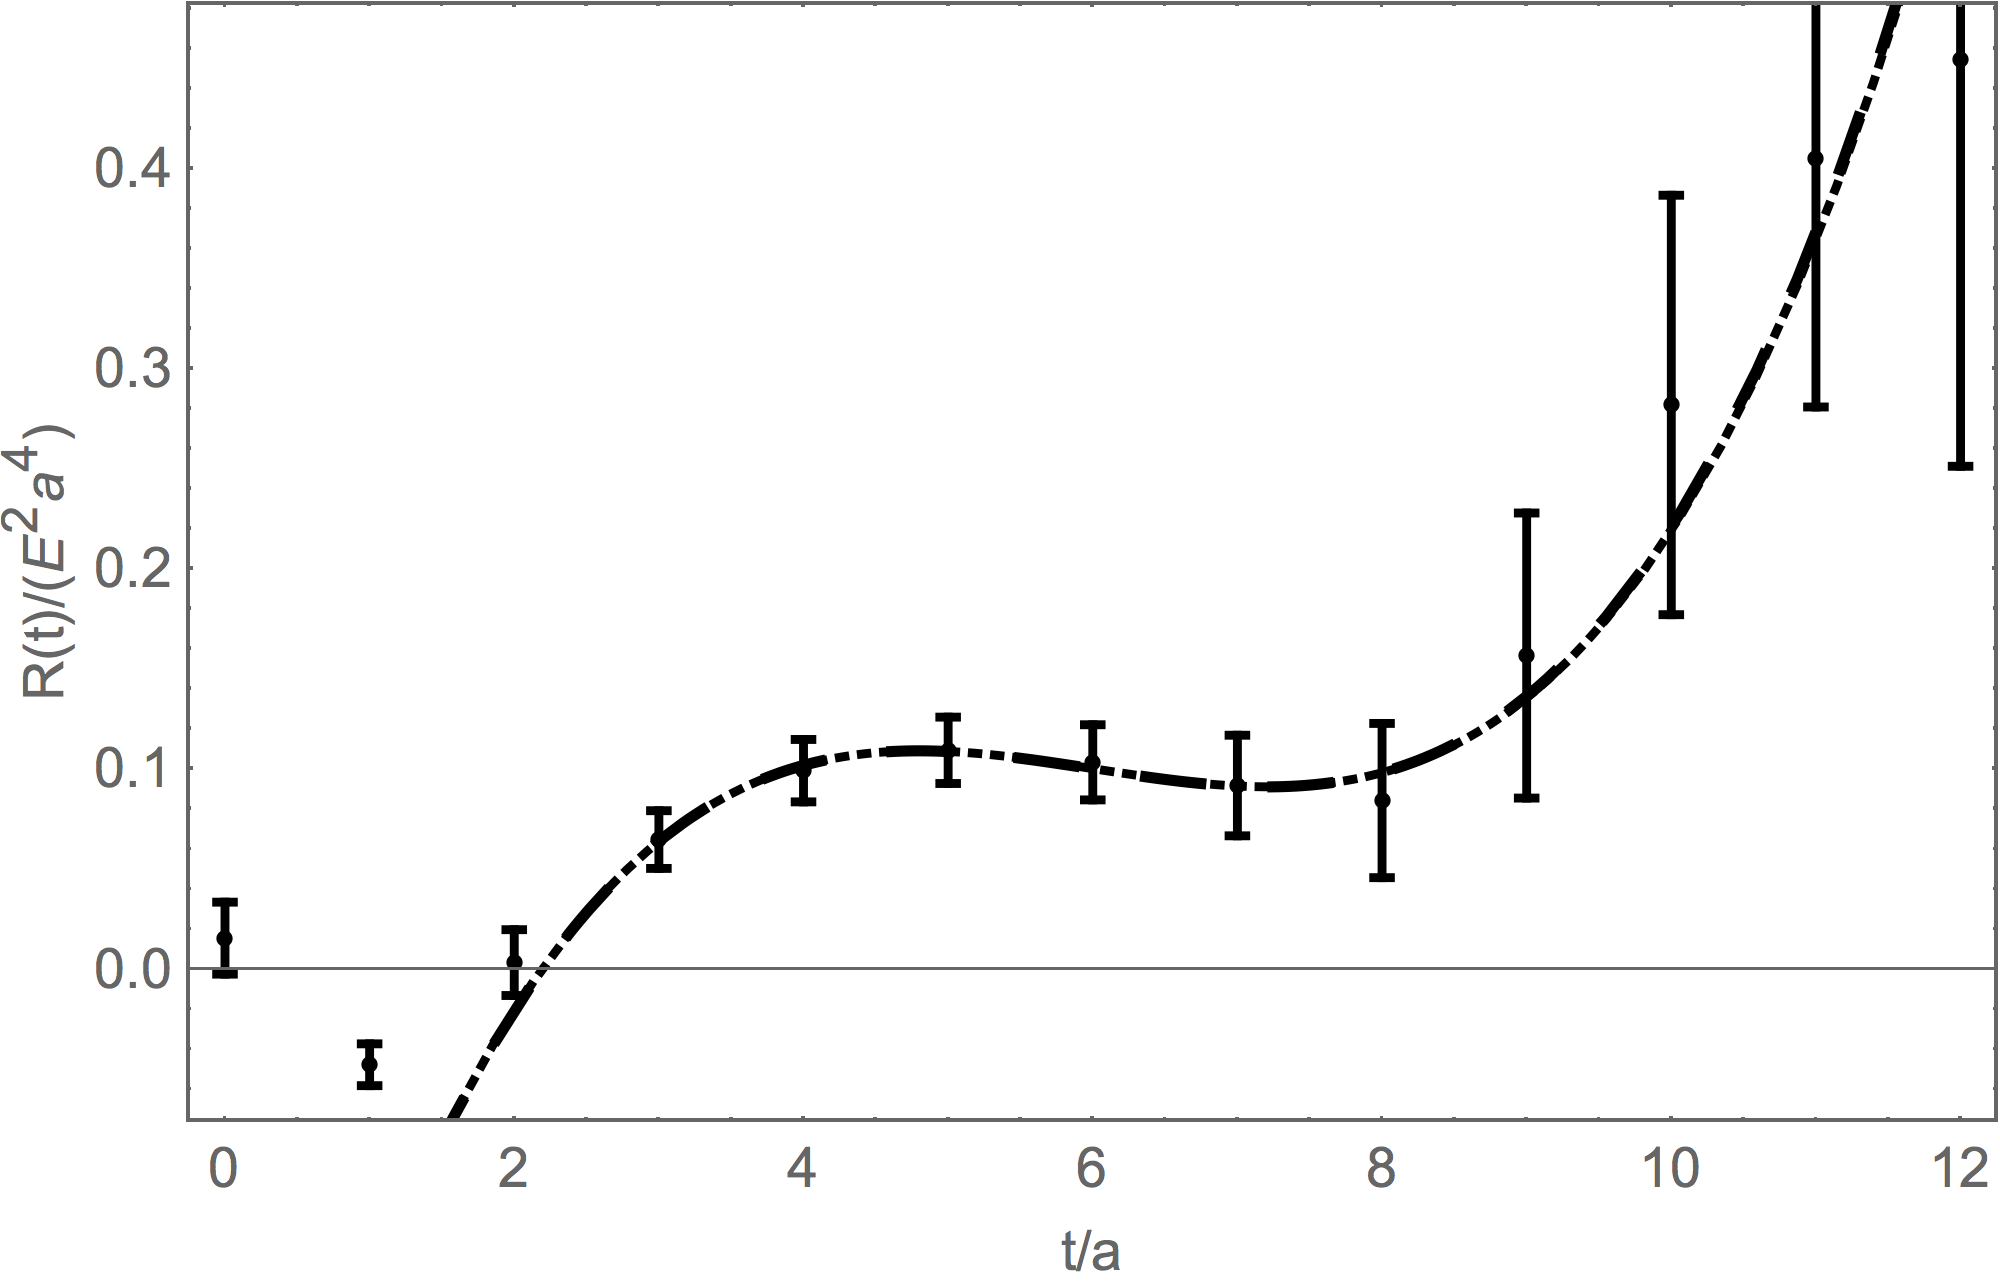
\includegraphics[width=.65\linewidth]{figures/shshQuadCS.png}\\
\caption{Correlator ratio $R_2(t)$ for the connected diagrams a), b), f), shown in Figure ~\ref{fig:diagrams}, in units of $E^2a^4$. A cubic form was fitted with (dotted line) and without (dashed line) a quadratic term.}
\label{fig:1walpha}
\end{figure}
%%%%%%%%%%%%%%%%%%%

Table~\ref{tab:1walphaconnected} shows the inflection points and extremal slopes. The inflection
point positions are compatible with $t/a=6$. The importance of the positions
of these points becomes apparent in light of the possible retardation effects,
which will be discussed below~\ref{retardation}.

%%%%%%%%Table 1-window connected Multi point%%%%%%%%%
\begin{table}[H]
\begin{center}
    \begin{tabular}{|l|l|l|}
    \hline
     Fit range   & 4 to 8   & 3 to 9  \\ \hline
     Inflection point ($t/a$) 		& 6.6(1.2)       	& 6.01(50)      \\ 
     						& 6.55(89) 	& 6.06(45)	\\ \hline
     Extremal slope with   		& -0.012(12)     & -0.0112(88)          \\ 
     a quadratic term [$a^3$]	& -0.016(11)	& -0.0147(87)	\\ \hline
     Extremal slope w/o   		& -0.012(10)     & -0.01123(95)   \\ 
     a quadratic term [$a^3$]	& -0.016(10)	& -0.0150(93)	\\ \hline
    \end{tabular}
\end{center}
\caption{Inflection points and extremal slopes for the $\chi^2$ cubic fits in the 1-window analysis for connected diagrams a), b), f), shown in Figure ~\ref{fig:diagrams}. \todo{results from reduced statistics are given in the lower lines}}
\label{tab:1walphaconnected}
\end{table}
%%%%%%%%%%%%%%%%%%%%%%%%%%%%%%%%%%%
 

The  electric polarizability from the 1-window
analysis is presented in Table~\ref{tab:1wElectricPolarizabilityConn}. 
These measurements are consistent with those presented in 
Table~\ref{tab:ConnectedPolarizabilities} for the 3-window analysis of the data.
Comparing these two result tables allows one to
identify smaller statistical errors in the 3-window analysis than in 
the 1-window counterpart. However, it is not guaranteed that the
correlator ratio $R_2(t)$ behaves in a purely cubic way, 
especially if scrutinized far away from the inflection point. \textcolor{red}
{In this regard, there is an unquantified systematic uncertainty in the 3-window analysis.}

%%%%%%%%%Static polarizability 1-window%%%%%%%%%%%%%%%
\begin{table}[H]
\begin{center}
    \begin{tabular}{|l||c|c||c|c||}
    \hline	& \multicolumn{2}{c||}{with quadratic term} & \multicolumn{2}{c||}{w/o quadratic term} \\ \hline
     Fit range [$t/a$)]						& 4 to 8 	& 3 to 9 	& 4 to 8 	& 3 to 9 \\ \hline 
     $\alpha_E$ [$10^{-4}$ $\text{fm}^3$]    		& 0.46(46)	& 0.43(34) 	& 0.46(39)	& 0.43(36) \\ \hline     
     $\alpha_E-\alpha_{FW}$ [$10^{-4}$ $\text{fm}^3$]& 0.69(46) 	&  0.65(34)	& 0.68(39) 	& 0.65(36) \\ \hline
    \end{tabular}
\end{center}
\caption{Static electric polarizability  $\alpha$ and reduced by the Foldy-Wouthuysen contribution $\alpha-\alpha_{FW}$ from the extremal slopes (1-window analysis, connected diagrams, $\chi^2$ fits) of the two fitting ranges in units of $10^{-4}$ $\text{fm}^3$. \todo{'point' results?}}
\label{tab:1wElectricPolarizabilityConn}
\end{table}
%%%%%%%%%%%%%%%%%%